%
% File naaclhlt2010.tex
%
% Contact: nasmith@cs.cmu.edu

\documentclass[11pt,letterpaper]{article}
\usepackage{naaclhlt2010}
\usepackage{times}
\usepackage{latexsym}
\usepackage{graphicx}
\usepackage{float}
\setlength\titlebox{6.5cm}    % Expanding the titlebox

\title{Implementing and Analyzing Feedforward Deep Neural Networks with Backpropagation}

\author{Andrew Dykman\\
  JHU LCSR MSE\\
  2632 Guilford Ave\\
  Baltimore, MD 21218, USA\\
  {\tt adykman3@jhu.edu}
  \And
  Greg Langer \\
  JHU LCSR MSE \\
  24 E. Preston St. \\
  Baltimore, MD 21202, USA\\
  {\tt glanger1@jhu.edu}}

\date{}

\begin{document}
\maketitle
\begin{abstract}
  We created a framework in Python to build and train configurable neural networks in order to understand the results of changing different parameters and hidden layer geometries. We trained our network to classify written digits from the MNIST data set by taking the greyscale pixel values as inputs. Using this framework, we explored the implications of building and training our neural network with different dimensions and learning rates, as well as experimenting with online, batch, and various mini-batch configurations. We comment on the effect these changes have on training time and test accuracy.
\end{abstract}

\section{Introduction and Background}
\subsection{Neural Networks}

The class of Neural Networks is a Universal Function Approximator [Hornik 1989] built from small modules modeled after neurons. These networks are implemented to solve problems throughout the machine learning community. Feed-forward neural networks, as implemented in this project, pass information from an input layer, through one or more hidden layers, and finally through an output layer. These are configured to solve a variety of machine learning tasks, including classification and regression. The hidden layers contain several perceptron-like modules which take the outputs of the previous layer (either the input layer or a previous hidden layer) and combine them while implementing a nonlinearity, which allows the class of neural networks to create a universal function approximator [Hornik 1989]. While initially these networks produce outputs akin to noise, by backpropagating the error (network prediction compared to ground-truth) the network learns an association from input to output and in many cases is able to produce better results than other techniques in machine learning and elsewhere [Goh 1995]. Our networks' neurons use logistic regression classifiers: modules which dot feature vectors (input) with weight vectors (learned parameters) and add a bias term. We then pass the result through a sigmoid function, which returns a value between 0 and 1. For this application we calculate error using squared difference between the output and the listed label.

Neural Networks can learn online, in mini-batches, or in full batches. Online training backpropagates after each example, slowly moving the network towards the problem spaces optima, but not necessarily moving directly towards the optima. Batch learning involves running the entire training data set through the network before changing the network. This guarantees the network will move directly towards the problem space's optima (at least, the one for the training set), with some trade-offs in update time and complexity. Mini-batches are a compromise, instead taking a subset of the training set each time, calculating the best update, and then backpropagating it. These terms are not unique to Neural Networks, and are used in most machine learning tools.

\subsection{Parameters}

There are many parameters to tune in a neural network, but we focused on three: hidden layer geometry, mini-batch size and learning rate.\\
Hidden layer geometry is the number of hidden layers and the number of nodes within these hidden layers. While the class of shallow neural networks is a Universal Function Approximator, in practical applications increasing the depth can achieve better accuracy using fewer nodes than shallower networks. The trade-off here is vanishing gradients. Backpropagation of error becomes more and more ephemeral as one goes back in the network, and often very small numbers are rounded to $0$ by a computer which can only represent discrete values. One strategy to combat this issue is auto-encoding: training the network one layer at a time to represent the initial data, then finally backpropagating after the entire network is built for fine-tuning. We experiment with hidden layer geometry in section 3.3.\\
Learning rate is the amount that we want the network to move each iteration. Large learning rates cause the network to converge to an answer faster, but often causes 'overshoots' akin to a golfer constantly putting over the hole. Dynamic learning rate algorithms like ADAM optimizer [Kingma 2015] attempt to solve this problem, but implementing it was out of scope for the time that we had.\\
Mini-batch size, as described above, is the number of examples attempted and rolled into each training iteration. This causes a trade-off between speed of convergence and accuracy, as larger batches have more accurate updates but update slower and are susceptible to more bugs (as we discovered).

\section{Implementation Details}

\subsection{Code}
Our code builds from $NeuralLayer$ objects. These layers contain a matrix of weights to transform inputs to neural potentials, and vectors of the potentials and activations. All vectors and matrices are numpy arrays to speed up processing. The neural layer object is able to forward propagate by multiplying inputs by the weight function, then putting the results through a sigmoid to create the activated outputs that will be passed to the next layer. The object is also able to backpropagate error terms from the layer it feeds forward to, altering its own weights at the specified learning rate and calculating the distribution of error for the layer that serves as its input in feed-forward mode.\\
These $NeuralLayers$ are organized into networks with our $NeuralNetwork$ class. The class holds a list of $NeuralLayer$ objects, as well as the learning rate. During training, the $NeuralNetwork$ takes the initial inputs and passes them to the first layer, and from there on iterates through the list, taking the outputs of each layer and feeding it into the next layer until the last layer provides the output. Then, the $NeuralNetwork$ calculates the difference between the output and the true label, and passes it backwards through the network, allowing the layers to alter their own weights and propagate error to the layer behind.\\
Our measurable error from ground-truth is calculated only at the final layer of our Neural Network. We use that measured error to adjust the weights between the final two layers of our network. In all previous layers, we need a way to quantify the error at each internal, unobserved node. Since we cannot directly measure error by calculating its deviation from ground-truth, we need a way to propagate that error backwards. We calculate it by distributing the error backwards so that nodes that contributed the most to the incorrect label are punished the most. The matrix equation we used to backpropagate was of the form: \\
$\delta^{(l)} = (W^{l,l+1})^T \delta^{(l+1)} * g`(p^{(l)})$,\\
where $\delta$ is the vector of error terms for a given layer, $l$ is the currently layer, $W$ is the weight matrix between layers $l$ and $l+1$, $g�$ is the derivative of the sigmoid function, and $p$ is the vector of potentials.\\
We train the $NeuralNetwork$ using our mnistNN.py and batchmnistNN.py (for online and batch training respectively) scripts. These load our pickled data and labels, create a $NeuralNetwork$ of the specified shape, and tell the $NeuralNetwork$ class to classify results. The result is then compared to the true label. If incorrect, the $NeuralNetwork$ is instructed to calculate and backpropagate the error. Additionally, after every 1000 examples data on error rates is recorded for data collection purposes. These scripts have command line configurations to change batch sizes, learning rate, and define error output file names.
\subsection{Data Preparation}
We used the MNIST handwritten digits dataset [LeCun] as it is easily available and a good experimental data-set for learning about neural networks. We converted the data to a numpy format using the code from [Larsson 2012], then changed the labels to a one-hot format and the image data to a 784x1 vector where all values are scaled from $0$ to $1$ (initially $0$ to $255$) and saved them using the pickle library. The data was split into train and test data sets initially, and we maintained this distinction throughout.
\subsection{Roadblocks}
Though we were ultimately successful in our implementation and testing, we did run into some roadblocks along the way. We ran into some problems constructing our our backpropagation algorithm. Initially we had trouble understanding the core of the math behind it. Once we got through that, we had some issues with the dimensionality of the vectors and matrices that we were multiplying, especially when considering adding in the bias terms. Once we finally got back propagation implemented, we initially neglected to add in an alpha value, so the learning rate was effectively equal to one. Once we recognized that mistake, we tried testing many different alphas to properly tune our neural network for different setups. After that we had to overcome the learning curve for implementing our own bash scripts, but after solving our syntactical and parsing errors, we ended up with a working pipeline for testing our networks with a range of parameters.
\subsection{Libraries}
Though we did not use any machine learning libraries for our project, we did make use of some standard Python libraries to help us along the way. The libraries we used for this project include Numpy for storing and multiplying data in vectors and matrices for forward and back propagation, Pickle to save and load data for access in multiple scripts, Scipy.stats for our logistic function, Argparse for integration with our bash scripts so we could test with different values and output graphs, and Matplotlib to automate the creation of graphs.

\section{Results}
This section will be split up into the independent experiments done: learning rate, batch size, and changing shape of the network. In all tests the networks saw the same data in the same order, and within each test the networks were trained for the same number of iterations.
\subsection{Online Learning Rate}

\begin{figure}[ht!]
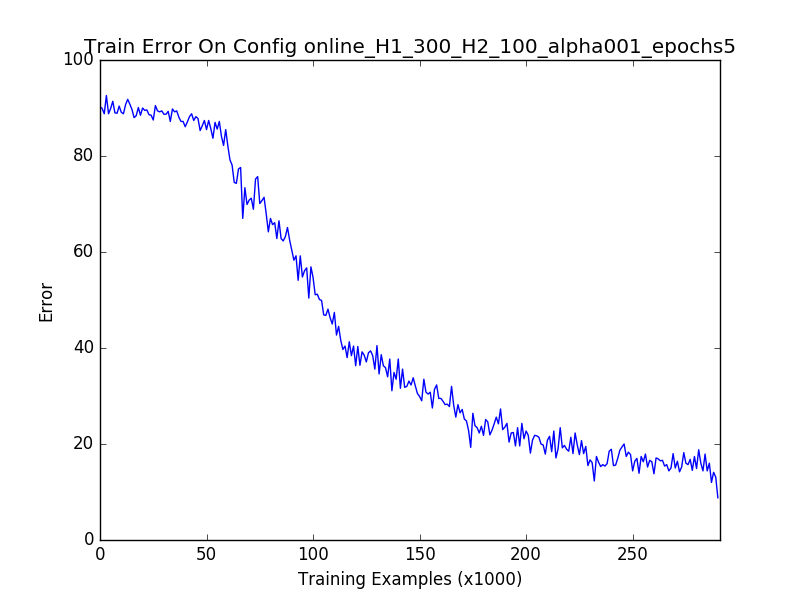
\includegraphics[width=0.5\textwidth]{../outputPlots/online_H1_300_H2_100_alpha001_epochs5.png}
\caption{Learning rate of $0.001$ with 2 hidden layers of size $(300, 100)$}
\end{figure}

\begin{figure}[ht!]
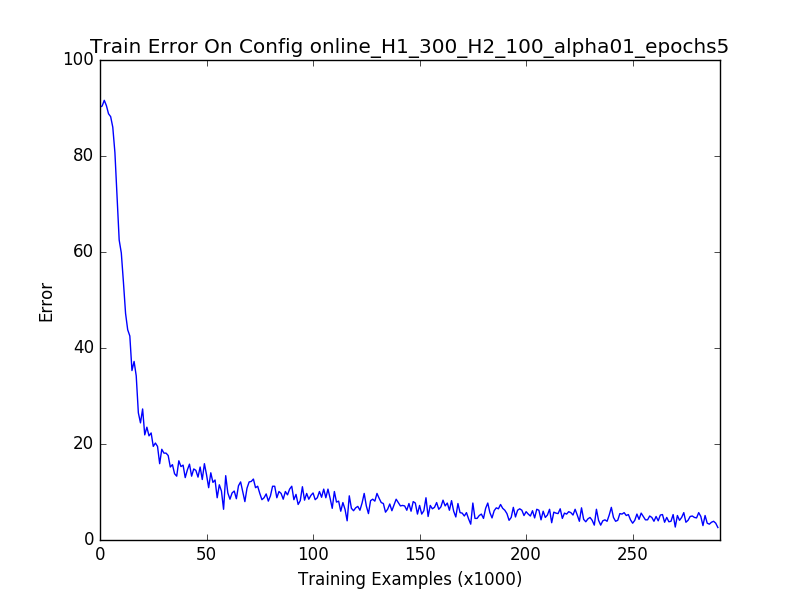
\includegraphics[width=0.5\textwidth]{../outputPlots/online_H1_300_H2_100_alpha01_epochs5.png}
\caption{Learning rate of $0.01$ with 2 hidden layers of size $(300, 100)$}
\end{figure}

\begin{figure}[ht!]
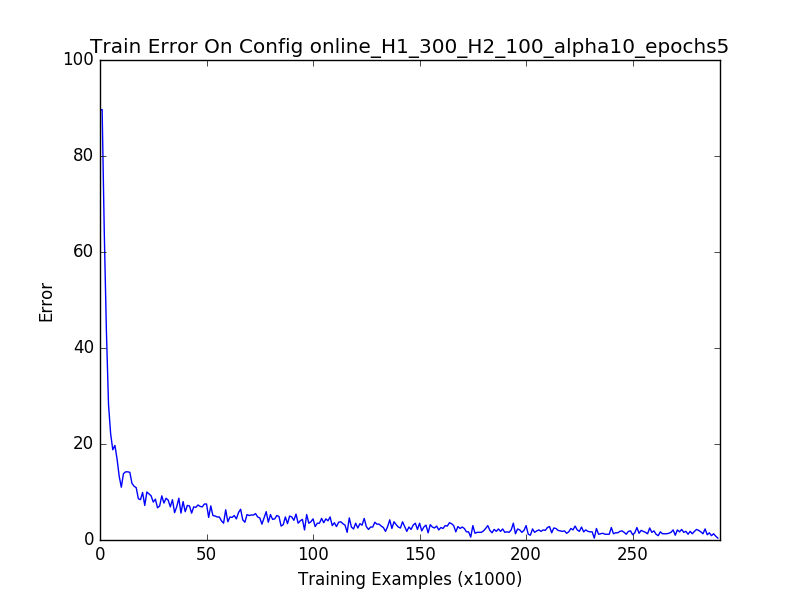
\includegraphics[width=0.5\textwidth]{../outputPlots/online_H1_300_H2_100_alpha10_epochs5.png}
\caption{Learning rate of $0.10$ with 2 hidden layers of size $(300, 100)$}
\end{figure}

The online learning rate experiment tested the difference in learning curves for networks with different learning rates, $0.001, 0.01, 0.03, 0.06, 0.10,$ and $0.20$, on a network with two hidden layers of size $(300, 100)$. Unsurprisingly, the tests with step sizes of $0.001$ and $0.01$ took the longest to converge (FIGURES 1, 2), with a fairly consistent increase in convergence speed as step size increased. However the final error varied greatly between tests. The smallest step, $0.001$, never reached convergence due to not having enough training epochs (FIGURE 1). That being said, the final error stays at a similarly low error ($<10\%$) from $0.01$ to $0.10$ (FIGURES 2, 3), before going back up at $0.20$. The fastest convergence to a sub-$10\%$ error rate came from the $0.10$ learning rate, and this makes sense for a relatively simple problem like the MNIST handwritten digit dataset. A more complex problem would likely take many more iterations and a more nuanced variable learning rate (only $300,000$ iterations were used total, and the network reached near-convergence in $50,000$). If we had more time to put into this project, we would set up runs for at least a million iterations, and repeat this experiment for multiple network shapes as well.

\subsection{Batch Size}

\begin{figure}[ht!]
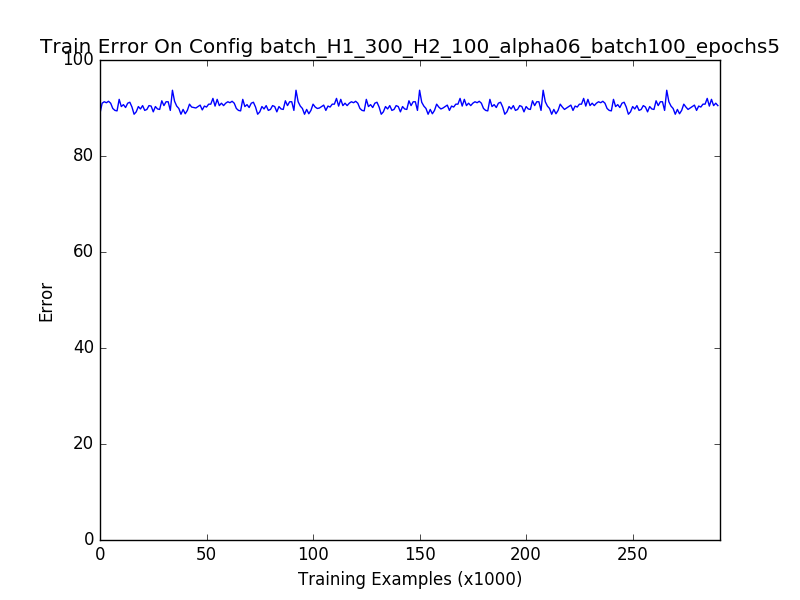
\includegraphics[width=0.5\textwidth]{../outputPlots/batch_H1_300_H2_100_alpha06_batch100_epochs5.png}
\caption{Batches of size 100, unsuccessful at achieving any training. Network has two hidden layers of size $(300, 100)$}
\end{figure}

\begin{figure}[ht!]
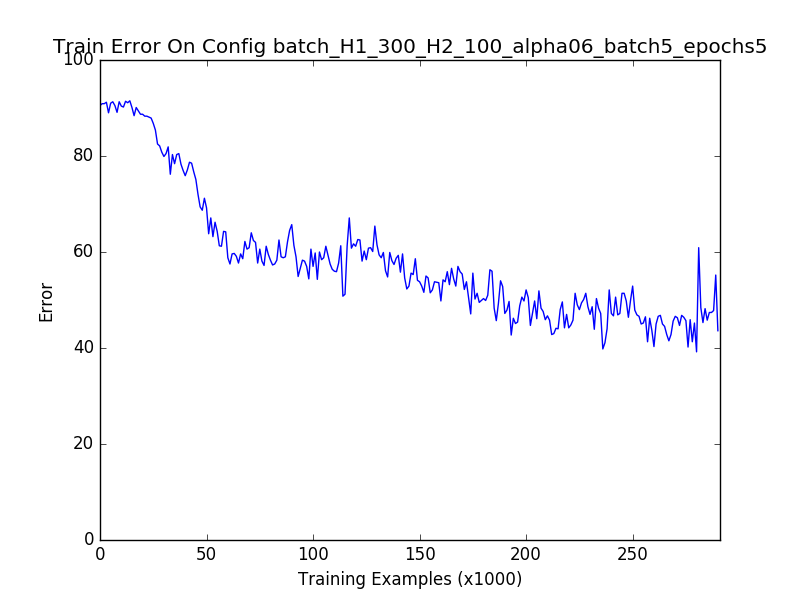
\includegraphics[width=0.5\textwidth]{../outputPlots/batch_H1_300_H2_100_alpha06_batch5_epochs5.png}
\caption{Batches of size 5, successful at classification to an extent. Network has two hidden layers of size $(300, 100)$}
\end{figure}

An experiment on batch size was attempted, but was ultimately not very informative. The premise was to use a network of hidden layers with size $300$ and $100$, a learning rate of $0.06$, and varying batch sizes. A batch of size $5$ (FIGURE 5) over $300,000$ examples did get to about $50\%$ error, and likely would have gone lower with more time. The rest of the tests (ex. FIGURE 4) with larger batches never dropped below chance ($90\%$ error) and we are not sure if this is due to a bug in our batch code, or an issue with our step size. Given more time for the project, we would spend significant time debugging the batch code and running for at least a million examples.

\subsection{Hidden Layer Geometry}

\begin{figure}[h!]
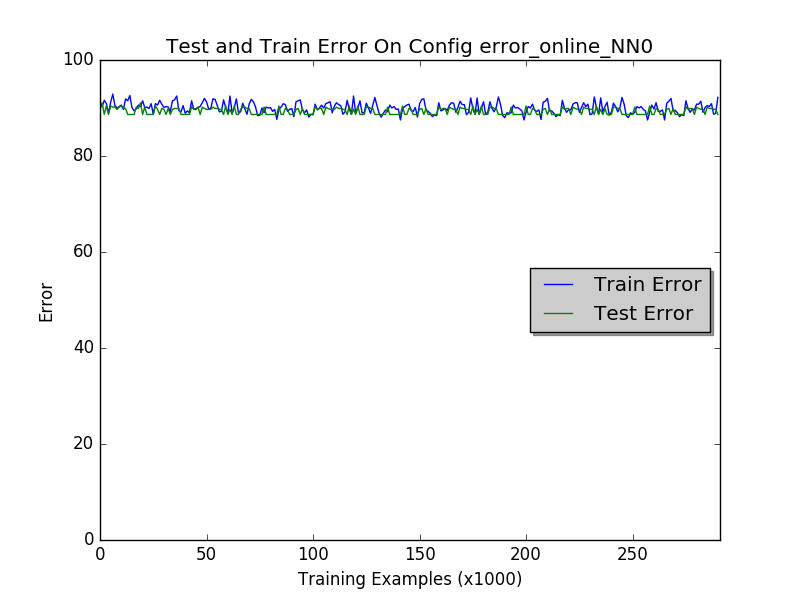
\includegraphics[width=0.5\textwidth]{../outputPlots/train_error_online_NN0.png}
\caption{Neural Network 0: Hidden Layers of Size$(350,175,85,40,20)$}
\end{figure}

\begin{figure}[h!]
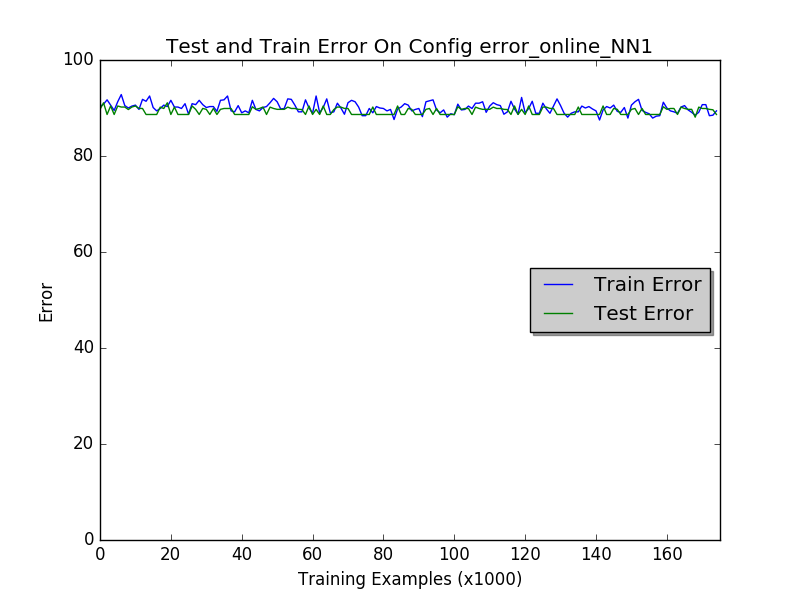
\includegraphics[width=0.5\textwidth]{../outputPlots/train_error_online_NN1.png}
\caption{Neural Network 1: Hidden Layers of Size$(300,150,75,40)$}
\end{figure}

\begin{figure}[h!]
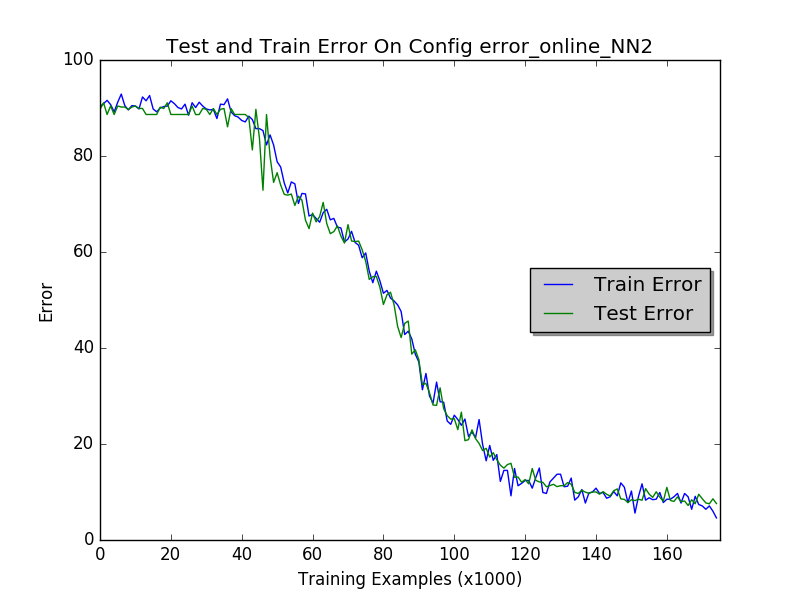
\includegraphics[width=0.5\textwidth]{../outputPlots/train_error_online_NN2.png}
\caption{Neural Network 2: Hidden Layers of Size$(280,130,60)$}
\end{figure}

\begin{figure}[h!]
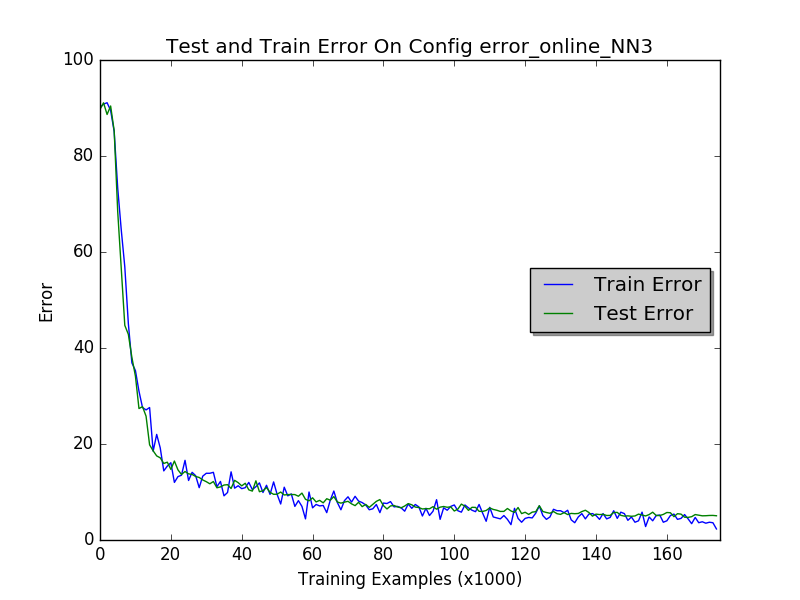
\includegraphics[width=0.5\textwidth]{../outputPlots/train_error_online_NN3.png}
\caption{Neural Network 3: Hidden Layers of Size$(250,100)$}
\end{figure}

\begin{figure}[h!]
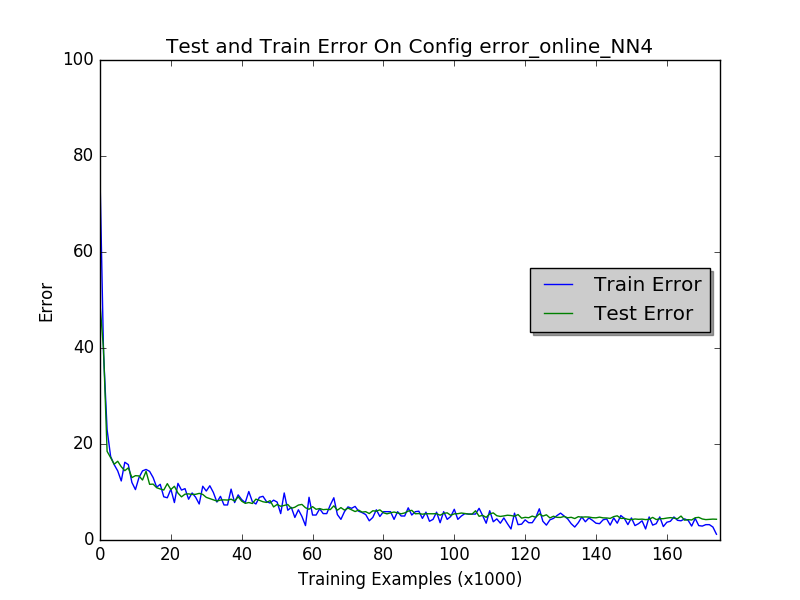
\includegraphics[width=0.5\textwidth]{../outputPlots/train_error_online_NN4.png}
\caption{Neural Network 4: Hidden Layers of Size$(175)$}
\end{figure}

In changing our Neural Network shape, we used 5 different geometries. Our five geometries of hidden layers were as follows, where each number represents a number of nodes in a hidden layer, so for example, $(250,100)$ has an input layer of image pixels, an output layer of size 10, and two hidden layers of size $250$ and $100$.\\
As you can see  (FIGURES 6, 7), our larger networks failed to learn anything useful, and the network accuracy achieved a success approximately as good as random guessing. We believe this is due to our networks being too large for standard backpropagation to be successful. As backpropagation goes further and further back, each node gets smaller and smaller $\delta$ terms, resulting in minimal changes to early weights in the system [Glorot 2010]. Since the first few layers do not learn anything useful, the following layers do not return intelligent results. In the next test (FIGURE 8), we can see that the network can finally learn something useful from the training data. In a future test, it would be interesting to give this network geometry more training examples to see how well it would converge. With even shallower networks (FIGURES 9, 10), we see rapid learning and stable convergence. We understand this to mean that shallower networks allow gradients propagating backwards to learn useful features without vanishing, and that it can learn the data quickly and get incrementally better over time.

\vspace{5 mm}

\section{Distribution of Time Spent on Project}
Out of the approximately 80 combined hours on this project, 45 hours were spent creating and debugging the neural network code, around 20 hours were spent designing tests, debugging the testing, and gathering data, and slightly over 15 hours were spent writing this paper.

In creating the neural network, we initially wanted to create a Network, Layer, and Neuron class. This took about 10 hours all told, but we realized that the extra computational time for function calls to the neuron class would not be worth the abstraction, and opted to vectorize neurons inside the layer instead. This set-up, including building the classes and implementing everything up to forward propagation took around 15 hours. The backpropagation, as described in Section 2.3 took another 20 hours between the two of us, as we had to understand the math, design the code, and debug it.

Once that was finished, we wanted to create automated bash scripts to try several configurations and record results. As most of the runs took close to an hour, we set up the scripts in advance and ran several experiments in a row overnight. Designing the ArgParse functionality, bash integration, and data set-up took 7 hours, and debugging the results (whether from crashed scripts or empty outputs) took up another few, though it is hard to pinpoint the exact time spent.

Finally, writing up this paper took around 15 hours, as we had to organize our thoughts, parse the generated data, and find good sources.


\section{Comparison to Proposal}
\subsection{Intended to Achieve}

Our first (and simplest) goal was to implement the feedforward part of a 2 layer neural network in an efficient and pythonic format. We achieved this goal unquestionably.\\
Our second goal was to implement the backpropagation portion of the same 2 layer neural network in an efficient and pythonic format. While this took much longer than expected, we definitely achieved this goal.\\
Finally we wanted to achieve $75\%$ accuracy, and in our best cases we got below $1\%$ train accuracy and below $4\%$ test accuracy.

\subsection{Expected to Achieve}

We expected to expand this project to create a flexible neural network with configurable numbers of hidden layers and depths. We did achieve this goal, but experienced an issue of vanishing gradients with larger networks. This was not an issue of the configuration, which was achieved, but if we were to put this into production we would need to build a more complex training routing, such as auto-encoding.

\subsection{Hoped to Achieve}

We hoped to implementing various deep learning set-ups and benchmark their success. We achieved this to some extent - we built these networks and ran our standard backpropagation algorithm on them, but did not find time to teach them using more complex techniques as noted above, such as auto-encoding.\\ 
We also hoped that if we had enough time we would be able to expand our training to accommodate the 26 letters of the alphabet as well. If we had more time we would have sought out training data for this.\\
The only significant change we made was our dataset source. Instead of using a set of 5000 instances from Andrew Ng, we used the much larger and higher quality MNIST dataset.

\begin{thebibliography}{}

\bibitem[\protect\citename{Kurt Hornik, Maxwell Stinchcombe, Halbert White}1989]{}
Kurt Hornik, Maxwell Stinchcombe, Halbert White.
\newblock 1989.
\newblock {\em Multilayer feedforward networks are universal approximators}, volume~2.
\newblock Elsevier, Amsterdam, Netherlands.\\

\bibitem[\protect\citename{{Robert Hecht-Nielsen}}1989]{}
{IEEE}.
\newblock 1989.
\newblock {\em Theory of the backpropagation neural network}.
\newblock IEEE, San Diego, CA.\\

\bibitem[\protect\citename{{A.T.C. Goh}}1995]{}
{A.T.C. Goh}.
\newblock 1995.
\newblock {\em Back-propagation neural networks for modeling complex systems}, volume~9.\\

\bibitem[\protect\citename{{Xavier Glorot, Yoshua Bengio}}2010]{}
{Xavier Glorot, Yoshua Bengio}.
\newblock 2010.
\newblock {\em Understanding the difficulty of training deep feedforward neural networks}, volume~9.
\newblock 13th International Conference on Artificial Intelligence and Statistics, Sardinia, Italy.\\

\bibitem[\protect\citename{{Diederik Kingma, Jimmy Ba}}2015]{}
{Diederik Kingma, Jimmy Ba}.
\newblock 2015.
\newblock {\em ADAM: A Method for Stochastic Optimization}
\newblock ICLR, San Diego, CA.\\

\bibitem[\protect\citename{Yann LeCun, Corinna Cortes, Christopher J.C. Burges}]{}
Yann LeCun, Corinna Cortes, Christopher J.C. Burges.
\newblock {\em THE MNIST DATABASE}
\newblock Google Labs New York, New York.
\newblock http://yann.lecun.com/exdb/mnist/\\

\bibitem[\protect\citename{Gustav Larsson}]{}
Gustav Larsson.
\newblock 2012.
\newblock {\em MNIST to numpy}
\newblock University of Chicago, Chicago, IL.
\newblock http://g.sweyla.com/blog/2012/mnist-numpy/\\


\end{thebibliography}

\end{document}
